\documentclass[12pt, titlepage]{article}

% Packages

\usepackage{booktabs}
\usepackage{tabularx}
\usepackage{float}
\usepackage{hyperref}
\usepackage{indentfirst}
\usepackage{listings}
\usepackage[round]{natbib}
\usepackage[usenames, dvipsnames]{color}
\usepackage{tikz}

% Setup

\hypersetup{
    colorlinks,
    citecolor=blue,
    filecolor=ForestGreen,
    linkcolor=MidnightBlue,
    urlcolor=blue
}

\lstset{
	basicstyle=\ttfamily\footnotesize
}

% Custom Commands

\newcounter{funCounter}
\newcounter{nonCounter}
\newcounter{pocCounter}

\newcolumntype{R}[1]{>{\raggedleft\let\newline\\\arraybackslash\hspace{0em}}p{#1}}
\newcolumntype{L}[1]{>{\raggedright\let\newline\\\arraybackslash\hspace{0em}}p{#1}}
\newcolumntype{C}[1]{>{\centering\let\newline\\\arraybackslash\hspace{0em}}p{#1}}

\newcommand\testTitle{NULL}
\newcommand\testCounter{NULL}

% Arguments
%    1 = {F, N, P} for functional, non-functional, and PoC respectively
%	 2 = Test name
%    3 = {Static, Dynamic}
%    4 = {Manual, Automatic}
%    5 = {Black, White}
%    6 = Initial state
%    7 = Input
%    8 = Output
%    9 = How the test will be performed
\newcommand{\test}[9]{	
	\begin{table}[H]
		\if#1F
			\stepcounter{funCounter}
			\renewcommand\testTitle{Functional }
			\renewcommand\testCounter{\thefunCounter} 
		\else
			\if#1N
				\stepcounter{nonCounter}
				\renewcommand\testTitle{Non-Functional }
				\renewcommand\testCounter{\thenonCounter} 
			\else
				\stepcounter{pocCounter}
				\renewcommand\testTitle{PoC }
				\renewcommand\testCounter{\thepocCounter} 
			\fi
		\fi
		
		\centering
		\def\arraystretch{1.6}
		\begin{tabular}{| R{7em} L{25em} |}
			\bottomrule
			\multicolumn{2}{| c |}{\textbf{#2} - \testTitle Test \# \testCounter} \\
			\hline
			\textit{Type:} & #3 / #4 / #5 Box\\
			\textit{Initial State:} & #6 \\
			\textit{Input:} & #7 \\
			\textit{Output:} & #8 \\
			\textit{Execution:} & #9 \\
			\toprule
		\end{tabular}
	\end{table}
	\smallskip
}

% Title Page Elements

\title{SE 3XA3: Test Plan\\Rogue Reborn}

\author{Group \#6, Team Rogue++\\\\
	\begin{tabular} {l r}
		Ian Prins & prinsij \\
		Mikhail Andrenkov & andrem5 \\
		Or Almog & almogo
	\end{tabular}
}

\date{Due Monday, October 31\textsuperscript{st}, 2016}

\input{../Comments}

\begin{document}

\maketitle

% Report outline

\pagenumbering{roman}
\tableofcontents
\listoftables
\listoffigures

% Revision Table

\begin{table}[bp!]
	\caption{\bf Revision History}
	\bigskip
	\begin{tabularx}{\textwidth}{p{3cm}p{2cm}X}
		\toprule {\bf Date} & {\bf Version} & {\bf Notes}\\
		\midrule
		10/21/16 & 0.0 & Initial Setup\\
		10/24/16 & 0.1 & Added Unit Testing and Usability Survey \\
		10/24/16 & 0.2 & Added Most of Section 2 \\
		10/24/16 & 0.3 & Added Section 1 \\
		10/26/16 & 0.4 & Added PoC tests \\
		10/26/16 & 0.4.1 & Added Test Template \\
		10/30/16 & 0.5 & Added Non-Functional Req. Tests \\
		10/30/16 & 0.5.1 & Added Bibliography \\
		10/31/16 & 0.6 & Added Names to Test Template \\
		\bottomrule
	\end{tabularx}
\end{table}

\newpage

% Report Content

\pagenumbering{arabic}

\section{General Information}
\label{section1}

	\subsection{Purpose}
		The purpose of this document is to explore the verification process that will be applied to the Rogue Reborn project.  Interested stakeholders are welcome to view and critique this paper to gain confidence in the success of the final product.  After reviewing the document, the reader should understand the strategy, focus, and motivation behind the efforts of the Rogue++ testing team.

	\subsection{Scope}
		This report will encompass all technical aspects of the testing environment and implementation plan, as well as other elements in the domain of team coordination and project deadlines.  The document will also strive to be comprehensive by providing context behind critical decisions, motivating the inclusion of particular features by referring to the existing \textit{Rogue} implementation, and offering a large variety of tests for various purposes and hierarchical units.  Aside from the implementation, the report will also discuss a relevant component from the requirements elicitation process (and its relevance to the testing effort).

	\subsection{Acronyms, Abbreviations, and States}
		
		\begin{table}[H]
			\centering
			\caption{\textbf{Table of Abbreviations and Acronyms}}
			\label{TableAbbreviations}
			\bigskip
			\begin{tabularx}{\textwidth}{p{3cm}X}
				\toprule
				\textbf{Abbreviation} & \textbf{Definition} \\
				\midrule
				GUI & Graphical User Interface\\
				IM & Instant Messenger\\
				LoS & Line of Sight\\
				PoC & Proof of Concept\\
				VPS & Virtual Private Server\\
				\bottomrule
			\end{tabularx}
		\end{table}

		\begin{table}[H]
			\centering
			\caption{\textbf{Table of Definitions}}
			\label{TableDefinitions}
			\bigskip
			\begin{tabularx}{\textwidth}{p{3.5cm}X}
				\toprule
				\textbf{Term} & \textbf{Definition}\\
				\midrule
				\textbf{Amulet of Yendor} & An item located on the deepest level of the dungeon that enables the player character to ascend through the levels and complete the game\\
				\textbf{Boost} & C++ utility library that includes a comprehensive unit testing framework\\
				\textbf{Frame} & An instantaneous ``snapshot'' of the GUI screen\\
				\textbf{Libtcod} & Graphics library that specializes in delivering a roguelike experience\\
				\textbf{Monochrome Luminance} & The brightness of a given colour (with respect to the average sensitivity of the human eye)\\
				\textbf{Permadeath} & Feature of roguelike games whereby a character death will end the game\\
				\textbf{Player Character} & Primary game character that is controlled by the user in Rogue Reborn\\
				\textbf{Rogue} & The original UNIX game developer in 1980 that initiated the roguelike genre\\
				\textbf{Roguelike} & Genre of video games characterized by ASCII graphics, procedurally-generated levels, and permadeath\\
				\textbf{Slack} & An online communication platform specializing in team and project coordination\\ 
				\bottomrule
			\end{tabularx}
		\end{table}	

		\begin{table}[H]
			\centering
			\caption{\textbf{Table of States}}
			\label{StateDefinitions}
			\bigskip
			\begin{tabularx}{\textwidth}{p{3.5cm}X}
				\toprule
				\textbf{State} & \textbf{Definition}\\
				\midrule
				\textbf{Developer State} & The file system state corresponding to the latest source code revision and compilation from the GitLab repository\\
				\textbf{Fresh State} & The file system state corresponding to a ``fresh'' Rogue Reborn installation\\
				\textbf{Gameplay State} & Any application state that reflects the actual gameplay\\
				\textbf{Generic State} & The file system state corresponding to a functional (working) installation of Rogue Reborn\\
				\textbf{High Score State} & Any application state that reflects the top high scores screen\\
				\textbf{Menu State} & Any application state that reflects the opening menu\\
				\textbf{Seasoned State} & The file system state corresponding to an installation of Rogue Reborn that already contains several high score records\\
				\bottomrule
			\end{tabularx}
		\end{table}	

	\subsection{Overview of Document}
		The early sections of the report will describe the testing environment and the logistic components of the Rogue Reborn testing effort, including the schedule and work allocation.  Next, a suite of tests will be discussed with respect to the functional requirements, non-functional requirements, and the PoC demonstration.  Upon discussing the relevance of this project to the original \textit{Rogue}, a variety of unit testing strategies will be given followed by a sample usability survey to gauge the interest and opinion of the Rogue Reborn game.  A breakdown of the sections is listed below:

		\begin{itemize}
			\item [] \hyperref[section1]{\S 1} Brief overview of the report contents
			\item [] \hyperref[section2]{\S 2} Project logistics and the software testing environment
			\item [] \hyperref[section3]{\S 3} Description of system-level integration tests (based on requirements)
			\item [] \hyperref[section4]{\S 4} Explanation of test plans that were inspired by the PoC demonstration
			\item [] \hyperref[section5]{\S 5} Comparison of the existing \textit{Rogue} to the current project in the context of testing
			\item [] \hyperref[section6]{\S 6} Outline of the approach to be implemented for unit testing  
			\item [] \hyperref[section7]{\S 7} Appendix for symbolic parameters and the usability survey
		\end{itemize}

\newpage
\section{Plan}
\label{section2}
		
	\subsection{Software Description}

	Initially, a large component of the testing implementation involved the usage of \textit{Boost}.  In general, Boost is regarded as an industry standard C++ utility library and comes packaged with a great deal of documentation ~\citep{BoostHome}.  However, this is a double-edged sword --- Boost is heavy, globally encompassing, and requires plentiful effort to properly setup.  The Boost library is suitable for projects spanning years with dedicated testing and QA teams.  Unfortunately, this is not the present condition of the Rogue Reborn project, and with the project nearing completion over the next month, the Rogue++ team agreed that it would be unwise to start using Boost.\\

	Instead, an alternative solution has been proposed: native test cases can be written in C++ to perform exactly the required tasks and nothing extra.  The details of this implementation will be explained in the following sections.

	\subsection{Test Team}

	All members of the Rogue++ team will take part in the testing procedure.  While Mikhail and Ian were assigned the roles of Project Manager and C++ Expert respectively, Ori was given the title of Testing Expert. Testing will be primarily monitored and maintained by Ori although every team member will contribute to the testing facilities.  The logic behind this rationale is that it would be desirable for the team member who wrote class $C$ to write the unit tests for the same class $C$.  Due to the dependency structure of the project's design, there will be cases where a unit test for one class will encompass a partial system test for another class.  These instances can be extrapolated from the class inheritance diagram.

	\subsection{Automated Testing Approach}

	There has been considerable effort expended towards automating project infrastructure components.  In the real world, any task that \textit{can} be automated, should be automated.  The steps that have been performed to reduce manual labour are as follows:

	\begin{itemize}
		\item Set up a GitLab pipeline for the project.  The pipeline is programmed to run a series of commands on an external VPS whenever a push is made to the GitLab repository.  Every run is logged and its history may be accessed at any time.
		\item Write a special makefile that produces 2 executables:
		\begin{enumerate}
			\item The Rogue Reborn game executable
			\item The project test suite.
		\end{enumerate}
		The details of this process will be described in the following sub-section.
		\item The team's primary method of communication is Slack: a cross-platform and programmer-friendly IM.  The Rogue++ team hooked the GitLab project repository to the team's Slack channel such that whenever the repository detects activity, a notification is sent to the channel.  This method greatly improves the team's awareness about each other's contributions and also facilitates communication about project-related inquiries.
	\end{itemize}

	\subsection{Testing Tools}

	The special makefile discussed above utilizes a phenomenon of C++ to perform the necessary steps.  First, it places \textit{all} source files into a dedicated folder to distinguish them between program files and test files; this is mandatory since there is an important relationship between the \textit{source} and \textit{test} classes.  Consider the diagram below:

	% Venn-diagram
	\begin{figure}[H]
		\centering
		\caption{\textbf{Source and Test Relationship}}
		\bigskip
		\label {Src-Test_Relationship}
		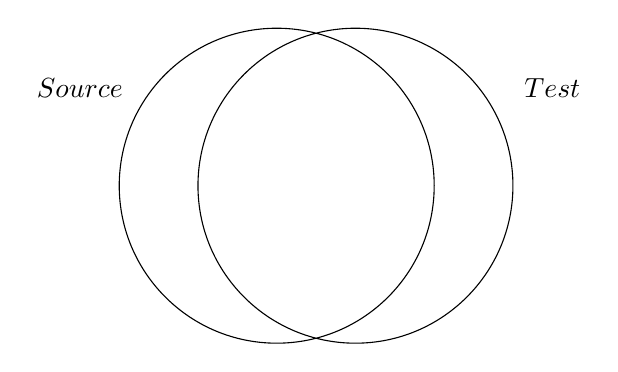
\begin{tikzpicture}[fill=white]
			% left hand
			\scope
			\clip (1,0) circle (1);
			\endscope

			% right hand
			\scope
			\clip (0,0) circle (1);
			\endscope

			% outline
			\draw 	(-0.5,0) circle (2) (-3,1)  node [text=black,above] {$Source$}
			 		(0.5,0) circle (2) (3,1)  node [text=black,above] {$Test$};
		\end{tikzpicture}
	\end{figure}

	\bigskip
	\bigskip

	As the diagram depicts, there are classes that are shared between both final programs.  In fact, the vast majority of classes fall in the center and are required by both the game executable as well as the testing component.  The files that are necessary for the tests but not for the source are, obviously, testing-related files that contain the test case implementations.  At the time of writing, there is only one file required by the source code that is not required by the test code: the source program entry (i.e. the C++ file that contains \lstinline$main()$).

	\bigskip

	The entire procedure of file collection, compilation, and separate linking is handled by the makefile, and is triggered by the \lstinline$make$ command.  From there, simply running \lstinline$Test.exe$ will trigger all of the pre-written tests.

	\bigskip

	There is also a plan to implement a Python script on the GitLab pipeline that will cause the build to fail if any of the tests do not pass.  It should be noted that, if a build fails, the pipeline not only reports the failure, but also logs the location of the failure down to the specific test case.  This will hopefully expedite the debugging process and lead to more responsible development further into the project timeline.

	\bigskip

	As an extra safety measure, the Rogue++ team will also be utilizing a tool called \textit{Valgrind} in the testing procedure.  Valgrind is a powerful analysis tool that tests the amount of memory a C++ program utilizes and detects memory allocation errors such as memory leaks ~\citep{ValgrindHome}.  C++, unlike Java and other high level languages, does not include a built-in garbage collector (otherwise there would be nothing left!) to give programmers total control over their application lifetime.  Consequently, it is a common mistake to accidentally leave unreferenced objects in memory and cause a memory leak in the program.\\

	At the time of writing, the Rogue Reborn application occupies approximately 1 MB of RAM during peak execution.  Although this is a minute quantity, memory leaks are representative of a larger issue: incorrect code!  By using Valgrind, the Rogue++ team will be able to detect the presence of these errors and indicate the direction of the next crucial bug fix.

	\subsection{Testing Schedule}
		
	The Gantt Chart can be accessed at \href{run:../../ProjectSchedule/Rogue.gan}{this location}.

\newpage
\section{System Test Description}
\label{section3}
	
	\subsection{Tests for Functional Requirements}

		%Dynamic 	Conduct test by running program
		%Static 	Conducted without running program (spell check)
		%~~~
		%Manual 	Actual human being has to decide if result is correct or not
		%Automatic 	Script
		%~~~
		%Black 		Decided on input and output
		%White 		Generate test cases based on code (Use code to make decisions)

		%123
		%initial state
		%input
		%output
		%how it will be performed

		\subsubsection{Basic Mechanics}

			\test{F}{New Game Start}{Dynamic}{Manual}{Black}{Fresh State}{A new game is started.}{The program is started.}{Either double-clicking the \lstinline$.exe$ or via terminal:

			\begin{center}
				\lstinline$./RogueReborn.exe$.
			\end{center}
			}

			\test{F}{Save Game}{Dynamic}{Manual}{Black}{Gameplay State}{Save command is given or the save key is pressed.}{A message indicating that the game has been saved is displayed to the user in the status area.}{A user will play the game and trigger the input sequence.  Note that this process can be verified by the Test \# 3.}

			\test{F}{Load game}{Dynamic}{Manual}{Black}{Gameplay State}{Load command is given or the save key is pressed.}{A message indicating that the game has been loaded is displayed to the user in the status area. The data model (level, player, monsters, etc.) is also updated to reflect the state changes.}{A user will play the game and trigger the input sequence to load and verify that it is in fact the same state that was previously saved.}

			\test{F}{Starting Statistics}{Dynamic}{Automatic}{Black}{Generic State}{A new game is started.}{The player character has the default starting equipment and statistics.}{This feature can be tested by analyzing the save file since it records all the necessary information about the player character.}

			\test{F}{Help Command}{Dynamic}{Manual}{Black}{Gameplay State}{The ``help'' command is given or the ``help'' key is pressed.}{The user is displayed a screen with a list of possible actions and other information.}{A user play the game and trigger the input sequence to display the ``help'' menu.}

		\subsubsection{Interaction}

			\test{F}{Detailer Player Information}{Dynamic}{Manual}{Black}{Gameplay State}{N/A}{Details about the player (level, health, known status effects, current depth, etc.) are displayed at the bottom of the screen in the area known as the \textit{Info Bar}.}{Rogue Reborn playtesters will be asked to answer basic questions about their player character at random intervals throughout the game.  To answer these questions, the user must refer to the Info Bar.}

			\test{F}{Environment Inspection}{Dynamic}{Manual}{Black}{Gameplay State}{The ``look'' key or command, and then an environment aspect character.}{After the input is supplied, a brief description of the environment aspect is displayed.  This can be limited to several words (e.g. ``This is an Emu'').}{Players will be told about the ``look'' key before their session and will have to employ it in order to gain information about their surroundings.}

			\test{F}{Pass Turn}{Dynamic}{Manual}{Black}{Gameplay State}{The ``wait'' key or command is pressed.}{All entities but the player engage in a turn by performing an action (as dictated by their respective AI).}{Players will be asked to skip their turn several times once an enemy is located (this tactic is used to ensure the player character delivers the first strike in a combat sequence).}

			\test{F}{Trap Activation}{Dynamic}{Manual}{Black}{Gameplay State}{A dungeon level that can generate traps (this only occurs at deeper levels).}{A message and a message describing the effect of the trap.}{Players will be asked to report the traps they encounter and the effect that was bestowed upon them upon activation.}

		\subsubsection{The Dungeon}

			\test{F}{Staircase Guarantee}{Dynamic}{Automatic}{Black}{Developer State}{A set of randomly generated dungeon levels.}{An indication of whether or not each dungeon contains a downwards staircase.}{Each generated level will be traversed using a simple graph discovery algorithm that tours every passable block; if no staircase is discovered, a flag is raised.}

			\test{F}{Level Accessibility}{Dynamic}{Automatic}{White}{Developer State}{A set of randomly generated dungeon levels.}{An indication of whether or not every dungeon level forms a strongly connected component.}{Each generated level will be traversed using a simple graph discovery algorithm that tours every passable block; if the number of discovered blocks is not equal to the number of blocks in the level, a flag is raised.}

			\test{F}{Line of Sight}{Dynamic}{Manual}{Black}{Gameplay State}{The player character is somewhere in the dungeon that is recognizable (i.e. not hidden) and is not blind.}{Visibility that depends on the player character's surroundings.  If the player character is in a room, they should be able to view the entire room.  If the player character is in a corridor, the player should only be able to view in surroundings within \hyperref[symbolicParameters]{VIEW\_DISTANCE} of their location.}{Users will be asked to assess the visibility standards.  Note that this is a bug-prone feature since many exceptions exist in the realm of the player character's current setting.}

			\test{F}{Amulet of Yendor}{Dynamic}{Automatic}{White}{Developer State}{Levels generated with a depth of \hyperref[symbolicParameters]{FINAL\_LEVEL}}{An indication of whether or not all generated levels contain the Amulet of Yendor on a reachable tile within the level.}{Each generated level will be traversed using a simple graph discovery algorithm that tours every passable block; if no Amulet is encountered, a flag is raised.}

			\test{F}{Searching \& Finding}{Dynamic}{Manual}{Black}{The player character in a dungeon beside a hidden door or passage.}{The player character activates the ``search'' command to search for adjacent hidden environment features.}{The door or passage is either revealed or remains hidden.}{Playtesters will be told before the game begins to occasionally look out for hidden doors; once discovered, the playtesters will document the number of searches that were required to reveal the hidden element.}

		\subsubsection{Equipment}

			\test{F}{Inventory Tracking}{Dynamic}{Manual}{Black}{Gameplay State}{New users are instructed to play the game with no special requirements.}{No users experiences a situation where the inventory screen does not represent their actual possessions.}{Users will be asked to laboriously maintain their inventory on a piece of paper and compare their copy to that of the game at various time intervals.}

			\test{F}{Identification \& Naming}{Dynamic}{Manual}{Black}{Gameplay State}{Users are instructed to pronounce the names of all items they collect.}{Users are unable to pronounce items they have yet to identify.}{Users will be asked to pronounce the generated names to the best of their ability to ensure they are nonsensical.}

			\test{F}{Armor \& Deterioration}{Dynamic}{Manual}{Black}{Gameplay State}{Users are assured that their armor is invincible.}{Users should complain that their armor loses effectiveness over time.}{Aquators and traps possess the capability to destroy player armor. Users should begin to encounter such setbacks (starting at level 6) and report their findings.}

		\subsubsection{Combat}

			\test{F}{Monster AI}{Dynamic}{Automatic}{White}{Developer State}{The position of the player character is transmitted to all monsters in a dungeon level.}{All aggressive monsters will calculate their respective paths and make progress towards the player character.}{An automatic script will be created to generate a level, spawn several monsters in the level, and then simulate a player character somewhere on the map.  From there, a traceback log of monster paths could be created and analyzed by having the player simulation repeatedly skip their turn.}

			\test{F}{Monster Attack Pattern}{Dynamic}{Automatic}{Black}{Developer State}{No target for monsters to attack.}{Monsters aimlessly wandering around.}{Similar to test \# 18, a level could be generated and populated with monsters; however, no player character location will be supplied to the level.}


	\subsection{Tests for Non-Functional Requirements}

		\subsubsection{Look and Feel Requirements}
			% Appearance
			\test{N}{Aesthetic Similarity Check}{Dynamic}{Manual}{Black}{Generic State}{Users are asked to rate the aesthetic similarity between \textit{Rogue} and Rogue Reborn.}{A numeric quantity between 0 and 10, where 0 indicates that the graphics are entirely disjoint and 10 indicates that the graphics are virtually indistinguishable.}{A random sample of users will be asked to play \textit{Rogue} and the Rogue Reborn variant for \hyperref[symbolicParameters]{PLAYTEST\_SHORT\_TIME} minutes.  Afterwards, they will be asked to judge the graphical similarity of the games based on the aforementioned scale.}

		\subsubsection{Usability and Humanity Requirements}
			% Ease of Use
			\test{N}{Interest Gauge Check}{Dynamic}{Manual}{Black}{Generic State}{New users are instructed to play Rogue Reborn.}{The quantity of time the user willingly decides to play the game.}{A random sample of users who are unfamiliar with \textit{Rogue} will be asked to play Rogue Reborn until they feel bored (or \hyperref[symbolicParameters]{MAXIMUM\_ENTERTAINMENT\_TIME} has expired).  Once the user indicates that they are no longer interested in the game, their playing time will be recorded.}

			% Personalization and Internationalization
			\test{N}{English Mechanics Check}{Static}{Manual}{White}{Developer State}{Rogue Reborn source code.}{An approximation of the English spelling, punctuation, and grammar mistakes that are visible through the GUI.}{All strings in the Rogue Reborn source code will be concatenated with a newline delimiter and outputted to a text file.  A modern edition of Microsoft Word from ~\citep{MicrosoftWord} will be used to open this generated text file, and a developer will manually correct all of the indicated errors that are potentially associated with a GUI output.}

			% Learning
			\test{N}{Key Comfort Check}{Dynamic}{Manual}{Black}{Generic State}{Users are asked to rate the intuitiveness of the Rogue Reborn key bindings.}{A numeric quantity between 0 and 10, where 0 indicates that the key bindings are extremely confusing and 10 indicates that the key bindings are perfectly natural.}{A random sample of users who are inexperienced with the roguelike genre will be asked to play Rogue Reborn for \hyperref[symbolicParameters]{SHORT\_TIME} minutes without viewing the in-game help screen.  Next, the key bindings will be revealed, and the users will continue to play the game for an additional \hyperref[symbolicParameters]{PLAYTEST\_SHORT\_TIME} minutes.  Afterwards, they will be asked to judge the quality of the key bindings based on the aforementioned scale}

		\subsubsection{Performance Requirements}
			% Speed and Latency
			\test{N}{Response Delay Check}{Dynamic}{Automatic}{White}{Generic State}{Users are instructed to play Rogue Reborn.}{A log of occurrences that indicate events where a computation that was initiated by a user input took an excessive quantity of time to execute.}{A random sample of experienced users will be asked to play a special version of Rogue Reborn for \hyperref[symbolicParameters]{PLAYTEST\_MEDIUM\_RANGE} minutes.  This edition will utilize a StopWatch implementation to measure the execution time of a computation, and if the computation exceeds \hyperref[symbolicParameters]{RESPONSE\_SPEED} milliseconds, the user action and the associated timestamp will be recorded in a log file.}

			% Precision or Accuracy
			\test{N}{Overflow Avoidance Check}{Static}{Manual}{White}{Developer State}{Rogue Reborn source code.}{All declarations of integer-typed variables.}{All occurrences of lines that match \hyperref[symbolicParameters]{REGEX\_INTEGER} (i.e., integer declarations) in the Rogue Reborn source code will be outputted to a file.  A group of Rogue++ developers will then review these declarations together and alter them if deemed necessary to avoid integer overflow issues.}

			% Reliability or Availability
			\test{N}{Crash Collection Check}{Dynamic}{Manual}{Black}{Generic State}{Playtesters are instructed to play Rogue Reborn for at least \hyperref[symbolicParameters]{PLAYTEST\_LONG\_TIME} hours.}{A collection of crash occurrences along with a detailed description of the failure environment.}{All Rogue Reborn playtesters will be required to play the game for at least \hyperref[symbolicParameters]{PLAYTEST\_LONG\_TIME} hours in total (spanned over multiple sessions if desired).  Every time the application crashes, the playtester must record the incident along with a description of the visible GUI state and the steps required to reproduce the failure.  After this data has been collected, the Rogue++ team will address every crash occurrence by either resolving the issue or confidently declaring that the event is irreproducible.}

			% Capacity
			\test{N}{Score Overflow Check}{Dynamic}{Dynamic}{White}{High Score State}{A high score record file containing a large quantity of entries.}{Rogue Reborn GUI displaying the top high scores.}{The Rogue Reborn developers will artificially fabricate a high score record file with at least \hyperref[symbolicParameters]{HIGH\_SCORE\_CAPACITY} + 2 records.  The game will then be played until the high score screen is revealed; only the top \hyperref[symbolicParameters]{HIGH\_SCORE\_CAPACITY} scores should be displayed.}

		\subsubsection{Operational and Environment Requirements}
			% Expected Physical Environment
			\test{N}{Processor Compatibility Check}{Dynamic}{Manual}{Black}{Fresh State}{Users are instructed to install and run Rogue Reborn on their personal machines.}{An indication of whether or not the game is able to successfully execute.}{A random sample of users with computers that are equipped with Intel x64 processors will be asked to download the latest Rogue Reborn distribution, perform any necessary installation, and then run the executable file.  The user will then report if the game was able to successfully run on their machine.}

			% Productization
			\test{N}{Streamline Distribution Check}{Static}{Manual}{Black}{Developer State}{Rogue Reborn distribution package.}{An indication of whether or not the distribution contains any files aside from the primary executable and the associated development licenses.}{The public distribution package will be visually inspected for extraneous files.}

		\subsubsection{Maintainability Requirements}
			% Maintenance
			\test{N}{Bug Productivity Check}{Static}{Manual}{Black}{Developer State}{All ITS issues labeled as bugs in the Rogue Reborn GitLab repository.}{An indication of whether or not all bug reports were closed within a month of their conception.}{The Rogue Reborn GitLab repository will be queried for all issues concerning bugs (which are denoted by a ``Bug'' label).  Next, a developer will manually verify that every closed bug fix request was resolved within a month of its creation.}

			% Adaptability
			\test{N}{Linux Compatibility Check}{Dynamic}{Manual}{Black}{Fresh State}{Users are instructed to run Rogue Reborn on their personal machine.}{An indication of whether the game can successfully execute.}{A random sample of users with computers that use a modern 64-bit Linux operating system will be asked to download the latest Rogue Reborn distribution, perform any necessary installation, and then run the executable file.  The user will then report if the game was able to successfully run on their machine.}

		\subsubsection{Security Requirements}
			% Integrity
			\test{N}{Illegal Records Check}{Dynamic}{Manual}{White}{Seasoned State}{A corrupted high score record file.}{Rogue Reborn GUI displaying the top high scores.}{The Rogue++ team will illegally modify a high score record file by manually altering or adding values such that the expected format or value integrity is violated.  These modifications should include negative high score values, missing text, and incorrect delimiter usage.  The game will then be played until the high score screen is revealed; all invalid record file contents should be ignored and amended in the next write to the record file.}

		\subsubsection{Legal Requirements}
			% Compliance
			\test{N}{License Presence Check}{Static}{Manual}{Black}{Developer State}{Rogue Reborn distribution package.}{An indication of whether or not the distribution is missing any mandatory license files.}{The original \textit{Rogue} source code hosted by ~\citep{BSDRogue} will be reviewed for legal requirements, and the public distribution package will be visually inspected to ensure that all mandatory license files are present.}

		\subsubsection{Health and Safety Requirements}
			% Seizure Prevention
			\test{N}{Seizure Prevention Check}{Dynamic}{Manual}{Black}{Developer State}{Two screenshots denoting the largest possible luminosity difference present between consecutive frames.}{The difference in luminosity between the two captured frames.}{After identifying the frame pair that is most likely to induce a seizure, the game will be played to reach the states that reflect each frame (this should be a brief process; no clever game model manipulation is required).  At the occurrence of each desired frame, the game screen will be captured and saved.  At this point, the average monochrome luminance across each frame will be calculated according to the formula \[L = 0.299R + 0.587G + 0.114B\] where $L$ is the luminance, $R$ is the red RGB component, $G$ is the green RGB component, and $B$ is the blue RGB component ~\citep{MonochromeLuminance}.  Finally, the absolute value of the luminance difference can then compared to \hyperref[symbolicParameters]{LUMINOSITY\_DELTA}.}   

\newpage
\section{Tests for Proof of Concept}
\label{section4}

	\subsection{Static Testing}
	
		\test{P}{Compile Test}{Static}{Automatic}{White}{Developer State}{Program source code.}{Program executable file.}{Run the makefile to verify that the program is able to successfully compile.}
		
		\test{P}{Memory Check}{Dynamic}{Manual}{White}{Generic State}{A brief but complete playthrough of the game.}{Breakdown of program memory usage.}{A playtester will briefly play the game while a developer uses Valgrind's memcheck utility to verify that program does not leak memory or utilize uninitialized memory.}

	\subsection{Rendering}
		\test{P}{Render Check}{Dynamic}{Manual}l{Black}{Gameplay State}{30-60 seconds of gameplay.}{The player character (along with any dungeon features) should be depicted at their  correct respective location with the correct glyph.  Additionally, the correct player statistics should be shown along the bottom of the screen.  The dialog box should correctly display the log and any prompts.}{A tester will manually play the game and verify that the GUI text is correct.}

	\subsection{Dungeon Generation}
		
		\test{P}{Dungeon-Gen Check}{Dynamic}{Manual}{Black}{Generic State}{Repeated restarts of the game}{Level should contain \hyperref[symbolicParameters]{ROOMS\_PER\_LEVEL} rooms, which should form a connected graph.}{A tester will manually start the game, briefly explore the level to verify correct generation, and then repeat this process until a sufficient level of confidence is achieved.}

	\subsection{Basic Movement}

		\test{P}{Movement Check}{Dynamic}{Manual}{Black}{Gameplay State}{Movement commands}{The player character should move about the level without clipping through walls, failing to walk through empty space, or jump to a tile that is not adjacent to their previous position.}{A playtester will manually walk through the level and visually verify correctness.}

	\subsection{Score File}

		\test{P}{Scoring File Check}{Dynamic}{Manual}{Black}{Menu State}{Enter a name, quit, restart the game, and then enter name again, and then quit.}{The first name should appear in both the first and second score screens; the second name should appear in only the second score screen.  Both records should have correct values for level, cause of death, and collected gold.}{A developer will manually perform the input sequence above and verify the output.  This should be tested both with and without an initial score file.}

	\subsection{Line of Sight System}

		\test{P}{Line of Sight Check}{Dynamic}{Manual}{Black}{Gameplay State}{Movement commands}{Screen should display correct portions of the level with the correct coloration schemes. This means that the player should be able to see the entirety of a room they are in or in the doorway of, and \hyperref[symbolicParameters]{VIEW\_DISTANCE} squares away if they are in a corridor.  Tiles that the player has previously explored but cannot currently see should be displayed in a dark shade of grey; tiles they have not yet been discovered should remain black and featureless.}{A developer will manually walk through the level, verifying that the above LoS rules are preserved (especially in edge cases like the corners of rooms and doorways).}

\newpage
\section{Comparison to Existing Implementation}	
\label{section5}
%How does it compare to the original and how does that help us test it
%Monster damage, etc.

	The original \textit{Rogue} is feature-full, and luckily, open source. This means that many, if not all of the features in Rogue++ can be tested in accordance with their similarity to the original game. Some examples are discussed below.\\

	An attempt has been made to replicate nearly one-for-one the items, loot, and treasure obtainable in the original \textit{Rogue}. Wands, staffs, rings, potions, ammunition, weapons, armor and more were all copied over with the same values in place. Regarding the items available for collection, players of the original game should feel right at home with the new Rogue++. Unlike some more modern games, the original \textit{Rogue} does not specify how effective an attack is besides hit or miss, as does Rogue++. This means that a player experienced with the original game may expect certain behavior out of a weapon or item, and find a difference in its effectiveness, despite the near one-to-one transition. This could stem from a variety of sources, perhaps most likely of which is a piece of code that does something unexpected, in an unexpected place.\\

	Another aspect of the game that was replicated as the source-code describes is dungeon generation. Of course, today we are using a more advanced data structure, with several capabilities that were not available for the C of 1980, but the idea behind the data structure is the same. The process followed for dungeon generation in 1980 was somewhat ill-conceived and convoluted. Despite this its discernible aspects were used as inspiration for the algorithm used in Rogue++. So while at the end of the day the two do not follow the same algorithm, the end result is close enough, and test cases are included to make sure that all properties of the old \textit{Rogue} are satisfied in Rogue++.\\

	Another way Rogue++ can be compared to the original \textit{Rogue} is by its controls. This is something that can be algorithmically tested, and guaranteed to function exactly as intended. Every key in \textit{Rogue} is mapped to a specific action, which can be replicated one-for-one in Rogue++. This kind of relationship makes testing easy, and makes implementation nearly trivial.\\

	The final comparison we will discuss is the environment in which each runs. The original \textit{Rogue} runs in the terminal, and still does so on *nix machines. Rogue++, however, runs in a window handled by libtcod (The Doryen Library). The differences may not mean much for a standard end-user, but for programmers this makes a world of difference. There are many dozens of different terminals, and each has its own special features, such as macros, special display characteristics, and more. The different environment may slightly alter response time, game speed, and several other factors. The differences between terminal Rogue and libtcod Rogue will be exactly the differences we will try to uncover with our tests and minimize with our implementation.

	
	
\newpage
\section{Unit Testing Plan}
\label{section6}
	
	After examining the boost library's utilities for unit testing, we have decided we will not use a unit testing framework for testing the product. We concluded that adding a framework would not make the work significantly easier, while reducing our flexibility and adding installation difficulties. Since we are not using a framework, drivers will be written by hand. Stubs will be produced when necessary to simulate system components. Since there are no database or network connections, stubs should hopefully be kept to a minimum. However, functions may be required to construct objects in states suitable for easy testing, for example creating a level or player with certain known properties, rather than by random generation.
	
	\subsection{Unit testing of internal functions}
		Internal functions in the product will be unit tested. This will be reserved for more complex functions so as to not waste development time unnecessarily. As complete code coverage is not a goal, generic code coverage metrics will not be used. Instead, care will be taken that complex functions are covered by unit tests. The following are examples of internal functions that are initial candidates for unit testing. Other functions will be added as necessary:
		\begin{itemize}
			\item The dungeon generation functions. The work of generating the dungeon is complex, but it is also easy to automate verification of dungeon properties such as a correct number of rooms, connectedness, compliance with formulas for item generation, presence or absence of certain key features such as the stairs connecting levels or the Amulet of Yendor in the final level.
			\item The keyboard input functions. As libtcod provides a Key struct which models keyboard input, we can mock/automate these functions. They are fairly complex, and since they return a pointer to the next desired state (similar to a finite state machine) we can easily verify their behavior.
			\item The item activation functions. For example it could be verified that when the player drank a potion of healing their health increased (if it was not at its maximum), that a scroll of magic-mapping is reveals the level, or that a scroll of identification reveals the nature of an item.
			\item The item storage functions. Each item is mapped to a persistent hotkey in the player's inventory. Certain items can stack with copies, reducing the amount of inventory space they take up, and how they are displayed. These factors make the inventory fairly complex. It is however easily verifiable, and automated testing can examine edge cases that would be impractical to test manually.
		\end{itemize}

	\subsection{Unit testing of output files}
		There is only one output file for the product, the high score file, which stores the scores in a csv format. The production and reading of this file can be unit-tested by verifying its contents after writing to it, and by providing a testing version of the file with known contents and verifying the function reads them correctly.

\newpage

\bibliographystyle{plainnat}

\bibliography{TestPlan}

\newpage
\section{Appendix}
\label{section7}

	This is where you can place additional information.

	\subsection{Symbolic Parameters}

		\begin{table}[h!]
			\centering
			\caption{\textbf{Symbolic Parameter Table}}
			\label{symbolicParameters}
			\bigskip
			\def\arraystretch{1.6}


			\begin{tabular}{| c | c |}
				\bottomrule
				\textbf{Parameter} & \textbf{Value} \\
				\hline
				ROOMS\_PER\_LEVEL & 9 \\
				FINAL\_LEVEL & 26 \\
				HEIGHT\_RESOLUTION & 400 \\
				LUMINOSITY\_DELTA & 0.5 \\
				MINIMUM\_ENTERTAINMENT\_TIME & 20 \\
				MINIMUM\_RESPONSE\_SPEED & 30 \\
				HIGH\_SCORE\_CAPACITY & 15 \\
				PLAYTEST\_SHORT\_TIME & 5 \\
				PLAYTEST\_MEDIUM\_RANGE & 10-20 \\
				PLAYTEST\_LONG\_TIME & 3 \\
				REGEX\_INTEGER & \lstinline$(char|int|long).*(,|;)$ \\
				START\_LEVEL & 1 \\
				VIEW\_DISTANCE & 1 \\
				WIDTH\_RESOLUTION & 1280 \\
				\toprule
			\end{tabular}
		\end{table}

\newpage
\subsection{Usability Survey Questions}

	\begin{enumerate}
		\item Is there any game feature you were unable to figure out how to utilize?
		\item How helpful was the help screen for you?
		\item Was there anything going on in the game that the interface failed to make clear to you or deceived you about?
		\item What common UI interactions did you find particularly lengthy?
		\item What aspects of the interface did you find unintuitive?
		\item How responsive was the interface?
		\item How easy was it to see everything that was going on?
		\item How effective are the graphics/symbols?
		\item Would an alternative input device such as a mouse make interacting with the interface easier for you?
		\item Is there any extra functionality you would like added to the interface?
		\item How difficult was it to learn the game? How much experience do you have with Roguelikes?
		\item How helpful was the original game manual?
		\item How pleasing was the color scheme?
		\item Was the font large enough for easy use?
		\item Were you able to learn the hotkeys easily?
	\end{enumerate}

\end{document}
